%!TEX root = ../template.tex
%%%%%%%%%%%%%%%%%%%%%%%%%%%%%%%%%%%%%%%%%%%%%%%%%%%%%%%%%%%%%%%%%%%%
%% chapter3.tex
%% NOVA thesis document file
%%
%% Chapter with a short latex tutorial and examples
%%%%%%%%%%%%%%%%%%%%%%%%%%%%%%%%%%%%%%%%%%%%%%%%%%%%%%%%%%%%%%%%%%%%

\typeout{NT FILE chapter3.tex}%

\makeatletter
\newcommand{\ntifpkgloaded}{%
  \@ifpackageloaded%
}
\makeatother


\chapter{Proposal}
\label{cha:Proposal}


This chapter details the choice and implementation of the proposed AI-driven tool, outlining all the important steps for it's development. From the laboratory processes, the data collection, to the AI model proposal itself that will be used to automate well-quarantining, the ultimate goal of this proposal is to develop a system that enhances the efficiency and accuracy of delivered sequencing results while reducing manual effort. By leveraging machine learning techniques, particularly unsupervised learning, the proposed tool will provide an automated approach to categorizing DNA samples based on their similarity according to multiple fields. This will address the current limitations of manual analysis, improving both speed and reliability in laboratory workflows.

The chapter begins with an overview of the laboratory processes involved in sequencing, including the preparation of samples in a 96-well PCR plate, and it's sequencing using the ABI3730xl DNA sequencer. Next, it discusses the data collection and storage procedures, emphasizing the structured format of sequencing outputs and metadata handling. Finally, it introduces the proposed AI model for use, detailing the methodology for clustering the DNA sequences and automating quality assessment.

\section{Laboratory Processes}
\label{sec:laboratory}

The laboratory processes described here are central to the generation of the data used in this work. These processes involve the handling of DNA samples, their preparation for sequencing, and the subsequent analysis of the results.

\subsection{Sample Preparation and Processing}
The laboratory workflow begins with the reception of DNA samples from various clients. These samples are organized into 96-well PCR plates, where each well is identified by a unique coordinate system: letters A to H for the rows and numbers 1 to 12 for the columns (Figure \ref{fig:96_well_plate}). This organization ensures traceability and efficient handling of multiple samples simultaneously. Samples from the same client are grouped together in neighboring wells, although not all wells need to be occupied for sequencing to proceed. Each plate must contain at least one control well.
\begin{figure}[H]
  \centering
  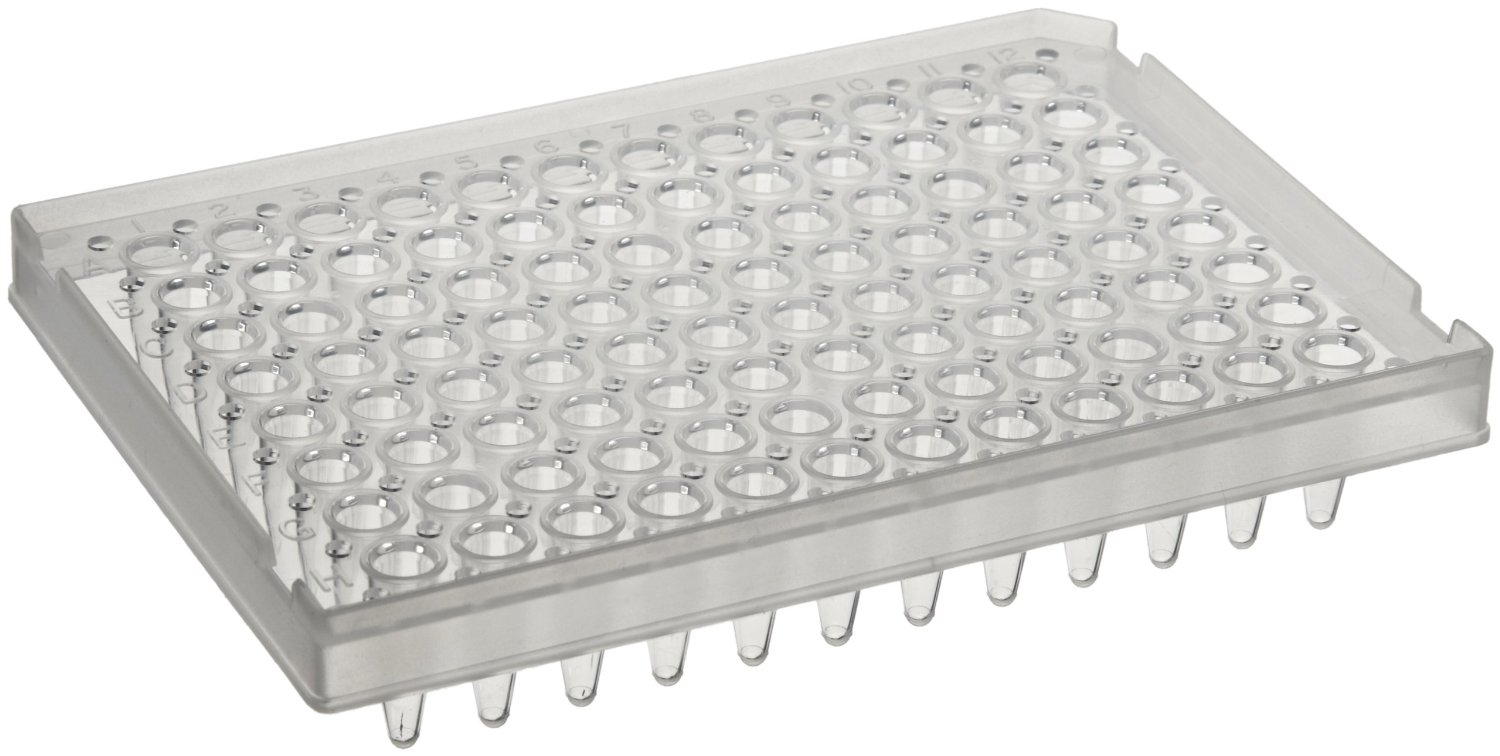
\includegraphics[width=0.8\textwidth]{96plate.png}
  \caption{A 96-well PCR plate.}
  \label{fig:96_well_plate}
\end{figure}


\begin{figure}[H]
  \centering
  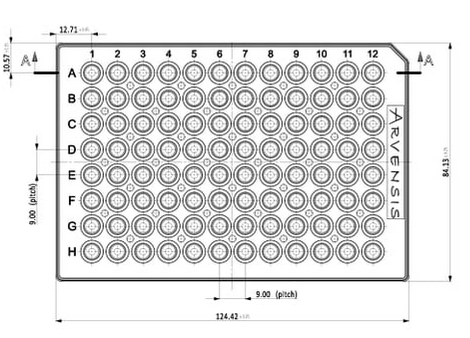
\includegraphics[width=0.8\textwidth]{platecoords.png}
  \caption{Structure and Organization of each PCR plate.}
  \label{fig:platecoords}
\end{figure}

Upon receipt, some samples require human intervention to prepare them for sequencing. For instance, samples with uneven DNA concentrations must be normalized to ensure consistent sequencing quality. Additionally, samples that do not include a primer must have the appropriate primer added by laboratory staff. These steps are critical to ensure the accuracy and reliability of the sequencing results. Each plate also contains 1 well reserved for solely for quality control, named \textit{Control}

Once prepared, these plates are then loaded into the ABI3730xl DNA sequencer, which includes DNA denaturation, primer annealing, extension with fluorescently labeled dideoxynucleotides, and capillary electrophoresis. The ABI3730xl sequencer then generates raw data files containing fluorescence intensity readings, which are subsequently processed to produce DNA sequence alignments.


\subsection{The ABI3730xl DNA Sequencer}
The ABI3730xl DNA sequencer is a high-throughput instrument widely used in genomics for Sanger sequencing. It automates the electrophoresis and fluorescence detection steps, corresponding to steps 3 and 4 of the Sanger sequencing process (Figure \ref{fig:sanger_steps}), allowing for the simultaneous processing of 96-well plates in a single run \cite{smith_capillary_sequencing,abi3730xl_overview}. By leveraging this technology, laboratories can achieve precise and efficient DNA sequencing. 
\begin{figure}[h]
\centering
\includegraphics[width=0.7\textwidth]{abi_3730xl_closed.png}
\caption{A closed ABI3730xl capillary electrophoresis DNA analyzer.}
\label{fig:abi_3730xl_closed}
\end{figure}

\begin{figure}[h]
\centering
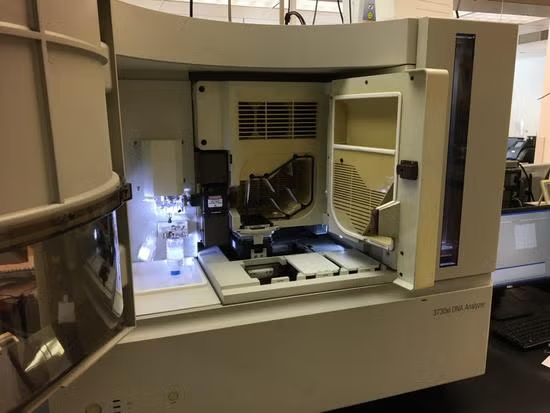
\includegraphics[width=0.7\textwidth]{abi_3730xl_opened.png}
\caption{An opened ABI3730xl capillary electrophoresis DNA analyzer.}
\label{fig:abi_3730xl_opened}
\end{figure}

\subsection{Data Generation \& Collection}

The effectiveness of any artificial intelligence model relies heavily on the quality and structure of the data used for training. In this work, the data originates from customer samples sequenced using the ABI3730xl DNA sequencer. Each well in a 96-well PCR plate generates multiple files, including raw fluorescence data, processed DNA sequences, and quality metrics. With each plate containing 96 wells and each well producing 6 distinct files, a single plate yields 576 files. Over time, as multiple plates are processed daily, this results in millions of files, forming a robust dataset for analysis.
The primary file types considered in this work include:

\begin{itemize}
  \item \textbf{Ab1 File}: Contains intensity readings for each of the four fluorescent dyes (A, T, C, G) used in Sanger sequencing, resulting in fluorescent traces. This file is optimized for long sequences (more than 500 bases).
  \item \textbf{Phd1 File}: Contains the DNA sequence derived from the fluorescence traces, along with quality scores and scan numbers.
  \item \textbf{Scf File}: Similar to .ab1 files, .scf files include quality information about the base calls, the chromatogram (also called the electropherogram), and the DNA sequence.
  \item \textbf{Seq File}: A plain text file containing the DNA sequence.
  \item \textbf{Qual File}: Includes the quality scores of each base in the DNA sequence.
  \item \textbf{Qualtrace File}: Contains additional information about the sequencing process, such as PeakStart, DyeSignal, Noise, and Spacing.
\end{itemize}

These files adhere to a strict naming convention: \textbf{ReactionID\_Pos\_DNAID+PrimerID}. 
For example, the file name \texttt{2338715\_A1\_AA8117+Clon\_2+ORB501} can be broken down as follows:
\begin{itemize}
  \item \texttt{2338715}: The unique reaction ID.
  \item \texttt{A1}: The position of the well in the plate (row A, column 1).
  \item \texttt{AA8117+Clon\_2}: The DNA ID, identifying the specific DNA sample.
  \item \texttt{ORB501}: The primer ID, which is optional as some customers provide samples with primers already included.
\end{itemize}
Thus, 6 files are generated for this specific well: 
\begin{itemize}
  \item \texttt{2338715\_A1\_AA8117+Clon\_2+ORB501.ab1}
  \item \texttt{2338715\_A1\_AA8117+Clon\_2+ORB501.phd.1}
  \item \texttt{2338715\_A1\_AA8117+Clon\_2+ORB501.scf}
  \item \texttt{2338715\_A1\_AA8117+Clon\_2+ORB501.seq}
  \item \texttt{2338715\_A1\_AA8117+Clon\_2+ORB501.qual}
  \item \texttt{2338715\_A1\_AA8117+Clon\_2+ORB501.qualtrace}
\end{itemize}

Other relevant and important information about each plate well, such as the associated \textbf{Client's Name}, \textbf{Sequence Length}, \textbf{Primer DNA Sequence} (If applied by the laboratory staff), and the \textbf{Control Well Status} is also available.  

\subsection{Manual Analysis}

After the data is generated, the laboratory staff manually handles quality checks on each plate individually, particularly for identifying possible fluorescence contamination and mismatches in sequencing results. This is a lenghty and thorough process that currently induces a bottleneck in the laboratory workflow. The main steps for quarantining wells are as follows:

\begin{itemize}
  \item \textbf{1. Control Well Check}: The laboratory staff begins by checking the \texttt{control\_well} for each plate. If the control well's \texttt{ok\_flag} is \texttt{NOT OK}, the entire plate is quarantined, as this indicates a problem with the sequencing process. If the control well passes the check, the process moves to the next step.
  \item \textbf{2. Sequence Clustering}: The sequencing software extracts the \texttt{ab1} files from each well (96 wells per plate) and clusters the sequences based on a minimum similarity of 66\%. This clustering is performed to group together DNA samples that are likely to belong to the same biological entity. Each cluster represents a set of related DNA sequences.
  \item \textbf{3. Cluster Verification}: The next step involves verifying these clusters for potential contamination or sequencing errors. Laboratory staff checks for two main conditions:
    \begin{itemize}
      \item \textit{Similar Sequences from Different Clients}: If samples from different clients have very similar DNA sequences, it may suggest fluorescence contamination, triggering a quarantine for further investigation.
      \item \textit{Same Primers with Different Sequences}: If different primers are associated with very similar DNA sequences, this could indicate contamination and thus requires quarantining.
    \end{itemize}
  \item \textbf{4. Forward and Reverse Sequence Matching}: DNA samples are analyzed based on forward and reverse sequencing. If a single base mismatch is detected in the same DNA sample (with matching \texttt{DNAID} and \texttt{primer\_id}), it is flagged for quarantine. In the case where a sample is processed with different primers, a variation in sequence is expected.
\end{itemize}

Sometimes certain samples do not appear to be contaminated, but the overall suspicion of such, or the poor quality presented, is enough to justify a quarantine, due to the importance of delivering accurate results.
After the anomalies are quarantined, these possibly contaminated samples are re-sequenced for an attempt at acquiring higher quality and accuracy, while the remaining samples are delivered to the client.

\section{Proposed Model \& Work}
\label{sec:model}

The importance of automating this manual process leverging AI-based technology now comes into place. Removing the need for manual individual analysis of all samples per plate is as important as delivring accurate results that would reflect a seamlessly human intervation.
The proposed work handles the early processes of processing the available data for model training, the model selection itself, and the validation and future deployability of the tool.

\subsection{Database Structure}
For model purposes, the database is structured with only relevant information, combining data derived from the majority of the introduced files with additional metadata. To simplify data management and improve query efficiency, a single table is proposed to store all relevant sequencing data and metadata. Below is the schema for this unified table:

\begin{table}[H]
  \centering
  \begin{tabular}{|l|l|p{8cm}|}
    \hline
    \textbf{Column Name} & \textbf{Data Type} & \textbf{Description} \\ \hline
    \texttt{Plate\_ID} & String & Unique identifier for each 96-well PCR plate. \\ \hline
    \texttt{Well\_POS} & String & Unique identifier for each well position (e.g., A1, B2). \\ \hline
    \texttt{Reaction\_ID} & String & Unique identifier for the reaction associated with the well. \\ \hline
    \texttt{DNA\_ID} & String & Identifier for the DNA sample. \\ \hline
    \texttt{Primer\_ID} & String & Identifier for the primer used (if applicable). \\ \hline
    \texttt{Client\_Name} & String & Name of the client associated with the sample. \\ \hline
    \texttt{Control\_Well\_Status} & String & Status of the control well (e.g., "OK" or "Quarantine"). \\ \hline
    \texttt{DNA\_Sequence} & Text & The DNA sequence derived from the `.seq` or `.phd.1` file. \\ \hline
    \texttt{Base\_Length} & Integer & The total number of bases of the DNA sequence. \\ \hline
    \texttt{Quality\_Scores} & Text & Quality scores for each base in the sequence (from `.qual` or `.phd.1` files). \\ \hline
    \texttt{Fluorescence\_Traces} & Text & Fluorescence intensity readings (from `.ab1` or `.scf` files). \\ \hline
    \texttt{PCR\_Size} & Integer & Size of the PCR product. \\ \hline
    \texttt{Purification\_Details} & Text & Information about the purification process. \\ \hline
    \texttt{Primer\_Sequence} & Text & Sequence of the primer used (if manually added by staff). \\ \hline
    \texttt{Date\_Processed} & Date & Date the plate was processed. \\ \hline
  \end{tabular}
  \caption{Unified Table Structure for Sequencing Data and Metadata.}
  \label{tab:unified_table}
\end{table}

This unified table structure ensures that all relevant information is stored in a single location, simplifying data retrieval and analysis. It includes fields for plate and well identification, sequencing data, quality metrics, and metadata, making it suitable for both clustering and contamination detection tasks.

For training, the data is consolidated into a unified table for efficient preprocessing and model development. For deployment, the AI-based tool is integrated directly with the company's servers to fetch and process data in real time.

\section{Data Preprocessing}
\label{sec:data_preprocessing}

To ensure optimal input quality for the AI-based model, multiple preprocessing steps are performed on the raw sequencing data. This includes sequence trimming, feature extraction, normalization of numerical features, and handling categorical/text-based attributes appropriately.

\subsection{Sequence Trimming}
Raw sequencing data contains noise, in the form of poor base quality, particularly at the start and end of sequences. This happens due to the 

\begin{figure}[h]
  \centering
  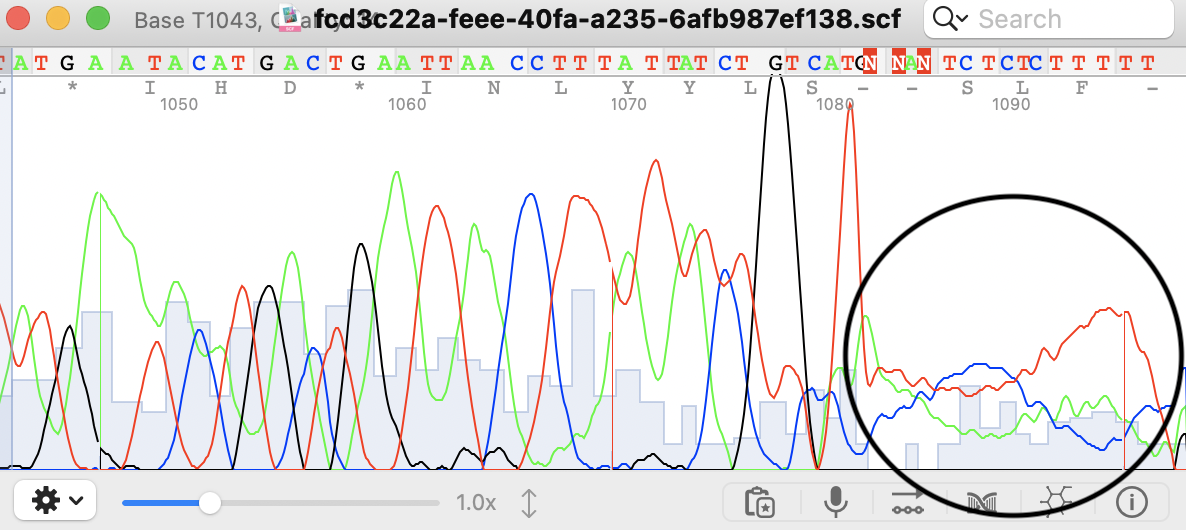
\includegraphics[width=0.7\textwidth]{noise1.png}
  \caption{Visualization of noise in the beggining of the DNA sequence, using 4peaks.}
  \label{fig:noise1}
\end{figure}

\begin{figure}[h]
  \centering
  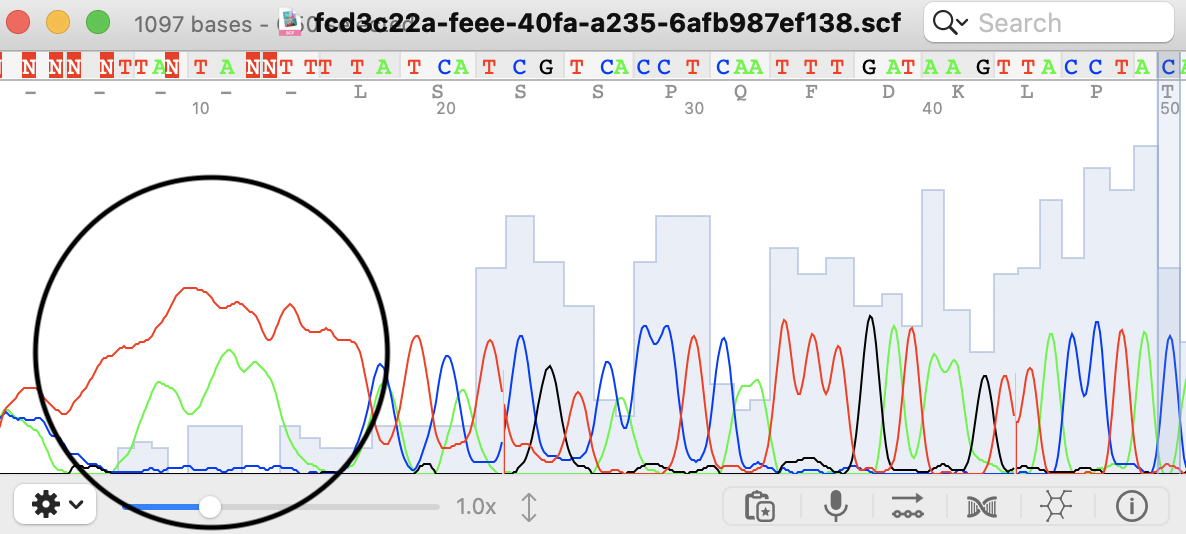
\includegraphics[width=0.7\textwidth]{noise2.png}
  \caption{Visualization of noise in the end of the DNA sequence, using 4peaks.}
  \label{fig:noise2}
\end{figure}

To improve downstream analysis, sequences are trimmed using the following criterion:

\begin{itemize}
    \item Bases are removed from the start and end of the sequence until \textbf{10 consecutive bases} have a \textbf{quality score} greater than 20.
    \item This ensures that only high-quality sequence regions are used for further processing.
\end{itemize}

The trimmed sequences are then stored for subsequent steps.

\subsection{Sequence Alignment Verification}
For DNA sequences that share the same DNA ID, alignment verification is performed to ensure consistency. This step helps detect sequencing errors and contamination by checking:

\begin{itemize}
    \item If forward and reverse sequences of the same DNA ID have mismatched bases, indicating sequencing inconsistencies.
    \item If sequences from different clients but within the same cluster show high similarity, suggesting potential contamination.
\end{itemize}

Alignment is performed using a pairwise sequence alignment algorithm, such as **Needleman-Wunsch** or **Smith-Waterman**, to ensure accurate comparison. These algorithms account for gaps and mismatches, allowing reliable verification of sequence integrity.

\subsection{Feature Extraction}
After trimming, relevant metadata and sequence-related features are extracted:

\begin{itemize}
    \item DNA sequence (A, T, C, G).
    \item DNA ID, Primer ID, Client Name, Plate ID, Plate Position, Plate Number, Date.
    \item Qualtrace data (e.g., capillary length, sequence length, etc.).
    \item Other well-related metadata.
\end{itemize}

\subsection{Normalization of Numerical Features}
To ensure that numerical features contribute equally to the model, normalization is applied where appropriate:

\begin{itemize}
    \item Quality scores, sequence lengths, and other quantitative features are scaled to a \textit{0-1 range} using \textbf{min-max normalization} or even \textbf{z-score normalization}.
    \item This prevents features with large values from dominating the model.
\end{itemize}

Categorical variables such as DNA ID and Primer ID are left in their original format or encoded as needed.
Even though \textbf{one-hot encoding} is commonly used in machine learning applications involving DNA sequences, in this context it is not necessary due to the unsupervised learning approach and the focus on sequence similarity rather than direct sequence classification \cite{bonat2023}. Instead, raw sequences are processed in their natural representation, ensuring efficiency and alignment with domain-specific methodologies.

\subsection{Final Processed Data}
The preprocessed data consists of:

\begin{itemize}
    \item Trimmed, high-quality DNA sequences.
    \item Aligned sequences for consistency verification.
    \item Normalized numerical metadata where applicable.
    \item Categorical information preserved in its original form.
\end{itemize}

This ensures that the AI model operates on well-structured and meaningful input data.

\section{Model Selection \& Development}
\label{sec:model_development}

The development of the AI-based tool involves selecting and training a model that can effectively automate the well-quarantining process. Given the lack of labeled anomalies, **unsupervised learning** techniques are the most appropriate choice. This section details the proposed models, their implementation, and the evaluation process.

\subsection{Model Selection}
The following unsupervised learning models are considered for the task:

\subsubsection{DBSCAN (Density-Based Spatial Clustering of Applications with Noise)}
- Purpose: To cluster sequences based on similarity and detect outliers (e.g., contamination).
- Advantages:
  - Does not require predefining the number of clusters.
  - Can identify noise and outliers effectively.
- Implementation:
  - Use sequence similarity (e.g. , based on k-mer frequencies or alignment scores) as the distance metric.
  - Tune the \textit{eps} (maximum distance between two samples to be considered neighbors) and \textit{min\_samples} (minimum number of samples in a neighborhood) parameters to optimize clustering performance.
- Output: Clusters of similar sequences and flagged outliers.

\subsubsection{Isolation Forest}
- Purpose: To identify sequencing errors and outliers.
- Advantages:
  - Efficient for high-dimensional datasets.
  - Focuses on isolating anomalies rather than profiling normal data points.
- **Implementation**:
  - Train the model on the feature matrix, using features such as sequence metrics, quality scores, and fluorescence traces.
  - Use the model to score each sample, with higher scores indicating a higher likelihood of being an anomaly.
- **Output**: Anomaly scores for each sample.

\subsubsection{Hierarchical Clustering}
- **Purpose**: To group sequences into a tree-like structure, allowing for flexible analysis at different levels of granularity.
- **Advantages**:
  - Provides a visual representation of clusters (dendrogram).
  - Does not require predefining the number of clusters.
- **Implementation**:
  - Use a distance metric such as sequence similarity or Euclidean distance on feature vectors.
  - Apply agglomerative clustering to build a hierarchy of clusters.
- **Output**: A dendrogram showing the relationships between sequences.

\subsection{Model Training}
- **Training Data**:
  - Use a subset of historical data for training the model.
  - Ensure the dataset includes diverse samples to improve generalization.
- **Training Process**:
  - Train each model on the preprocessed feature matrix.
  - Use cross-validation to evaluate model performance and avoid overfitting.
- **Hyperparameter Tuning**:
  - Use grid search or random search to optimize hyperparameters (e.g. , \textit{eps} and \textit{min\_samples} for DBSCAN).
  - Evaluate performance using metrics such as silhouette score (for clustering) and precision/recall (for anomaly detection).

\subsection{Model Evaluation}
- **Clustering Accuracy**:
  - Evaluate clustering performance using metrics such as **Adjusted Rand Index** (ARI) or **Silhouette Score**.
  - Compare the model's clusters with manual annotations (if available) to assess accuracy.
- **Anomaly Detection**:
  - Evaluate anomaly detection performance using metrics such as **precision**, **recall**, and **F1-score**.
  - Use historical contamination cases as a benchmark to validate the model's predictions.
- **Error Rate in Base Pair Matching**:
  - Measure the error rate in base pair matching by comparing the model's results with manual verification.
  - Calculate the **false positive rate** and **false negative rate**.

\subsection{Iterative Improvement}
- **Feedback Loop**:
  - Collaborate with laboratory staff to validate the model's predictions and refine it based on their feedback.
  - Incorporate additional features or adjust preprocessing steps as needed.
- **Model Updates**:
  - Periodically retrain the model using new data to ensure it remains accurate and up to date.
  - Use version control (e.g., Git) to manage changes to the model and deployment pipeline.

\section{Deployment Strategy}
\label{sec:deployment}

For deployment, the AI tool must integrate seamlessly with the company's infrastructure to provide real-time analysis of sequencing data. The following steps outline the deployment strategy:

\subsection{Real-Time Data Fetching}
- **Method**:
  - Use a file monitoring tool (e.g., `inotify` on Linux or `Watchdog` in Python) to detect new sequencing files in the company’s


  \subsection{Model Selection}
  The core requirement of the system is to automate the comparison of DNA sequences while integrating relevant metadata such as client identifiers, primers used, and sequencing run details. To achieve this, multiple unsupervised learning approaches are considered, each addressing different aspects of the verification process.
  
  \subsubsection{DBSCAN (Density-Based Spatial Clustering of Applications with Noise)}
  DBSCAN is selected as a candidate model for sequence clustering and anomaly detection due to its ability to identify patterns in data without requiring a predefined number of clusters. This characteristic makes it well suited for grouping DNA sequences with varying degrees of similarity while simultaneously detecting potential sequencing errors or contamination.
  
  The distance metric for DBSCAN will be derived from sequence alignment scores or k-mer frequency representations, ensuring biologically meaningful clustering. Hyperparameters such as \textit{eps} (maximum neighborhood distance) and \textit{min\_samples} (minimum points per cluster) will be optimized to enhance performance. The expected outcome of this model is the formation of distinct sequence clusters, with outliers flagged for further review.
  
  \subsubsection{Isolation Forest}
  Isolation Forest is considered for its effectiveness in detecting anomalies within high-dimensional datasets. By recursively partitioning the feature space and measuring how easily a sample is isolated, the model can identify sequencing errors or inconsistencies that deviate from expected patterns.
  
  Feature extraction will incorporate sequence-based attributes such as GC content, read quality scores, and fluorescence intensity deviations. The model will be trained on historical sequencing data, with an anomaly score assigned to each sample. Sequences with high anomaly scores will be flagged as potential errors requiring further validation.
  
  \subsubsection{Hierarchical Clustering}
  Hierarchical clustering provides an alternative approach to sequence grouping, offering a hierarchical representation of sequence relationships. This method is particularly advantageous in cases where sequences exhibit varying levels of similarity, allowing for flexible thresholding when defining cluster membership.
  
  Pairwise similarity metrics will be computed using sequence alignment or feature vector distances, followed by agglomerative clustering. The resulting dendrogram will serve as an interpretable visualization of sequence relationships, aiding in the refinement of clustering thresholds.
  
  \subsection{Model Training}
  The training phase will leverage historical DNA sequencing data to construct and optimize the proposed models. The dataset will encompass a diverse range of sequences to ensure robustness across different sequencing conditions.
  
  Prior to training, feature engineering will be conducted to transform raw sequencing data into a structured format suitable for analysis. The training process will involve multiple iterations of model refinement, incorporating techniques such as cross-validation to assess generalization performance.
  
  Hyperparameter tuning will be performed using methods such as grid search or Bayesian optimization, with evaluation metrics tailored to each model type. For clustering models, performance will be assessed using the silhouette score and Adjusted Rand Index (ARI), while the effectiveness of anomaly detection models will be measured through precision-recall metrics.
  
  \subsection{Model Evaluation}
  To ensure the reliability of the proposed system, a rigorous evaluation framework will be implemented. The performance of clustering models will be validated by comparing automated groupings against manually verified sequence clusters. Similarly, the accuracy of anomaly detection models will be benchmarked against known contamination cases, with precision, recall, and F1-score serving as key evaluation metrics.
  
  An additional layer of evaluation will involve assessing the model’s ability to detect errors in base pair matching, comparing automated results with manual verification outcomes. False positive and false negative rates will be quantified to determine the reliability of the system in identifying sequencing errors.
  
  \subsection{Iterative Improvement}
  Given the complexity of DNA sequence verification, an iterative approach will be adopted to refine model performance. A feedback loop will be established in collaboration with laboratory staff, enabling continuous validation of model outputs and adjustments to preprocessing strategies as necessary.
  
  Periodic retraining will be conducted using newly acquired sequencing data to maintain model accuracy over time. Furthermore, a version control system will be implemented to track modifications to the model architecture and hyperparameter configurations, ensuring reproducibility and traceability.
  